We have come to the best part of the paper. Making money. Many people you see in reality taking poses by their huge mansions and supercars. Majority of it is all fake. There have been many people that actually made money investing in bitcoin when it was not even known to the public (majority of people). Some guys back in the day mined $x$ amount of bitcoin to buy a slice of pizza. In today's time that $x$ amount of bitcoins are worth millions of dollars.
There is no theoretical way of getting a huge Return on investment (ROI) greater than 7\% in few hours (getting a ROI of 7\% could take months/days/years to gain in a stock market) but in crypto the ROI ranges $\% \in [0,100]$ in days ,weeks or months. A ROI of 7\% is a good enough ROI to make a good profit in trading. When you see bitcoin mining pools offering a ROI of 200\% or unrealistic gains you can be sure that is a scam. Let us say if we buy some bitcoin? As bitcoin is highly volatile maybe we can make money? I will prove to you below you wont make much money trading crypto currency. Mining is the best way to get into crypto. \\ 

In this chapter you will learn how to make money by mining bitcoin.
\begin{enumerate}
\item Basic calculations of crypto    
\item What is crypto mining?
\item What equipment is required to get started?
\item Converting our crypto assets to fiat money.
\end{enumerate}

\subsection{Basic calculations of crypto}

Consider the market chart for Bitcoin to South African rand:

You can get this chart just typing the following search query in Google: \\

$C_1 to C_2$ \\ 

where $C$ is a currency unit.

Example: \\

BTC to ZAR \\

to produce the market graph in Google.

\begin{figure}[H]
\centering
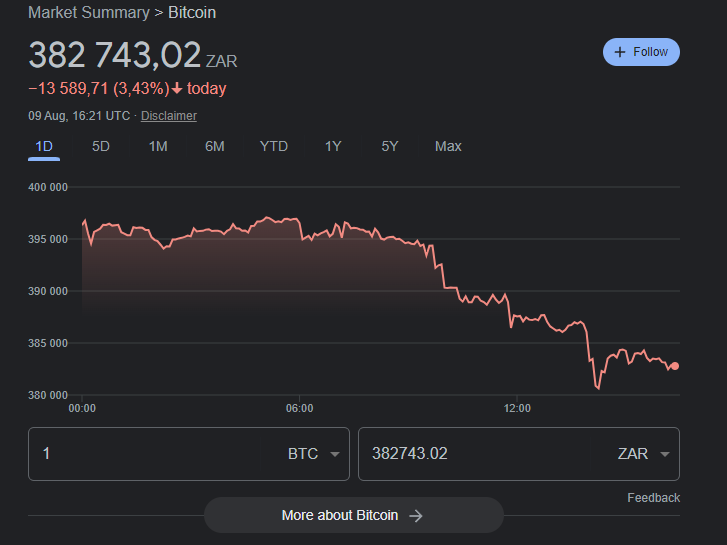
\includegraphics[width=0.6\textwidth]{images/btcmarket.png}
\caption{The market chart for BTC to ZAR}
\label{fig:bitcoin-market-chart}
\end{figure}

Given: 
$x$ is the amount of bitcoin you have. \\

R$382 742.02$ is the current price of 1BTC to ZAR. \\

Let us assume you have $x=$0.0026 bitcoins. \\

Our value in ZAR will be = $0.0026 * 382 742.02$ = R1000 \\

Let us now denote 1BTC is R500000 for a given day as it is volatile. \\
 
Our ZAR Wallet balance is determined by $0.0026 * 500000$ = R1300 \\

Our ROI is given by the formula:
\begin{equation}
    ROI = \frac{InvestmentGains-InvestmentCost}{InvestmentCost}
\end{equation}

$ ROI = \frac{1300-1000}{1000}$ = 30\% gain \\

While your ROI is high you can also lose your money like that.

As you can see we have made a 30\% gain in our ZAR wallet as crypto is volatile we have our good days and bad days but you the owner of the wallet can sell anytime as you please.

\subsection{What is crypto mining?}
Cryptocurrency mining, or cryptomining, is a process in which
transactions for various forms of cryptocurrency are verified and
added to the blockchain digital ledger. Also known as cryptocoin mining,
altcoin mining, or Bitcoin mining (for the most popular form of 
cryptocurrency, Bitcoin), cryptocurrency mining has increased both as a
topic of interest and an activity as cryptocurrency usage itself has 
grown exponentially in the last decade.

Bitcoin mining is the process by which new bitcoins are entered into circulation. It is also the way the network confirms new transactions and is a critical component of the blockchain ledger's maintenance and development. "Mining" is performed using sophisticated hardware that solves an extremely complex computational math problem. The first computer to find the solution to the problem receives the next block of bitcoins and the process begins again.

Cryptocurrency mining is painstaking, costly, and only sporadically rewarding. Nonetheless, mining has a magnetic appeal for many investors who are interested in cryptocurrency because of the fact that miners receive rewards for their work with crypto tokens. This may be because entrepreneurial types see mining as pennies from heaven, like California gold prospectors in 1849. And if you are technologically inclined, why not do it?

The bitcoin reward that miners receive is an incentive that motivates people to assist in the primary purpose of mining: to legitimize and monitor Bitcoin transactions, ensuring their validity. Because many users all over the world share these responsibilities, Bitcoin is a "decentralized" cryptocurrency, or one that does not rely on any central authority like a central bank or government to oversee its regulation. \\

In this paper I will be introducing your to NiceHash that connects sellers or miners of hashing power with buyers of hashing power. Buyers select the crypto-currency that they want to mine, a pool on which they want to mine, set the price that they are willing to pay for it, and place the order. This order is then forwarded to everyone who is connected to NiceHash with NiceHash Miner or other mining hardware (like ASICs). The computing power you provide will fulfil the buyer's order and you get paid for this service. You are basically selling processing power to companies.

\begin{figure}[H]
\centering
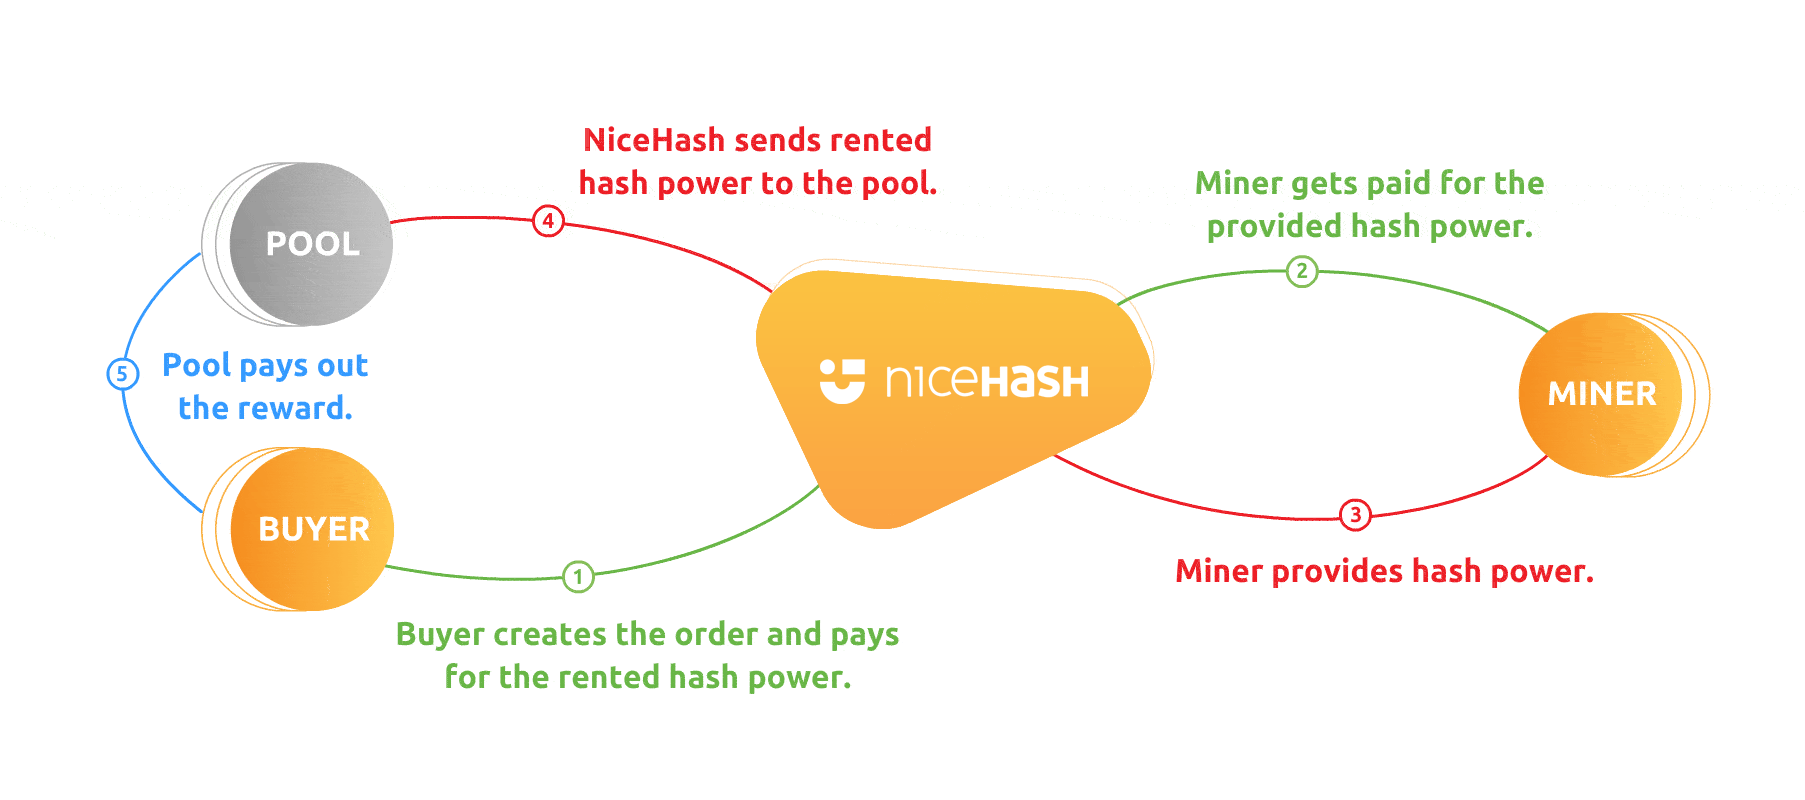
\includegraphics[width=0.8\textwidth]{a9ba234e12f0782b3184.png}
\caption{NiceHash Business Model}
\label{fig:nicehash}
\end{figure}

\subsection{Mining with NiceHash}

\subsubsection{Getting started with your computer and NiceHash} 
Consider a typical computer what does it consist of? I have indicated with a * the bare minimum to get a running computer.

\begin{enumerate}
\item \textbf{CPU*} (A central processing unit, also called a central processor, main processor or just processor, is the electronic circuitry that executes instructions comprising a computer program. The CPU performs basic arithmetic, logic, controlling, and input/output operations specified by the instructions in the program.)
\item \textbf{RAM*} (Random Access Memory, also called Random Access Memory (RAM), is a computer memory device that stores data in main memory. RAM is volatile, meaning that it is not preserved when a computer is shut down or rebooted. RAM is used to store data that is needed by the CPU to execute instructions. RAM is also used to store data that is needed by the CPU to execute instructions.)
\item \textbf{Motherboard*} (The motherboard is the main part of a computer that connects the CPU and other components to the computer's main power supply. The motherboard contains the main power supply, the CPU, and other components that make up a computer.)
\item \textbf{Hard Drive*}  (A hard drive is the hardware component that stores all of your digital content. Your documents, pictures, music, videos, programs, application preferences, and operating system represent digital content stored on a hard drive. Hard drives can be external or internal.)
\item \textbf{Graphics Card} (A graphics card is a computer peripheral that is used to display graphical images on a computer screen.)
\item \textbf{Operating System*} (An operating system is a computer program that manages the overall operation of a computer.)
\item \textbf{Power Supply*} (A power supply is a device that supplies power to a computer.)
\end{enumerate}

For mining you need a GPU (Graphical Processing Unit). A GPU is a computer peripheral that is used to perform graphics processing but in this case for mining it is used to solve algorithm problems for a reward.

Theoretically, the more processing power you have, the more you can process therefore the more money/reward/crypto you make.

So you can get started if you have a computer with a CPU, RAM, Motherboard, Hard Drive, Graphics Card, Operating System and Power Supply. Most importantly you need a GPU. \\

Now in a typical computer setup you can only have one/two GPU's at a time. That is your constraint.

\begin{figure}[H]
\centering
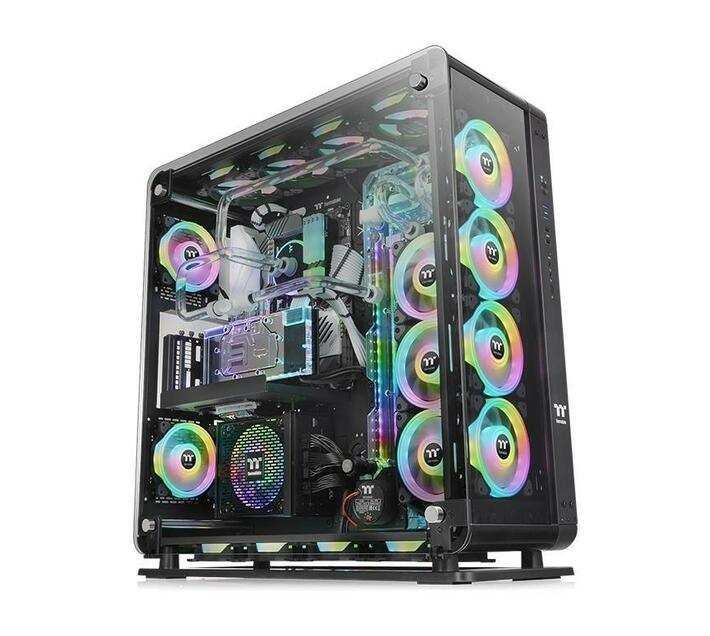
\includegraphics[width=0.8\textwidth]{51396074-6368-43c5-bcbf-1caca6d7a5f3-qpn13_large.jpg}
\caption{Gaming PC Rig}
\label{fig:pc}
\end{figure}


Different GPUs wields different rewards. For example a GeForce RTX 3080 has a higher reward than a GeForce RTX 3060ti.

If you want to play around and experiment with your own PC mining. Install NiceHash and run the miner tool. NiceHash provides you with a GUI that you can use to set up your mining and also provides you with a crypto wallet.

When you have done experimenting with your system. You can move on building a rig to support 8 GPUs+ at once.

\subsubsection{Building a mining rig and working out profitability} 

For a mining rig you dont need a strong CPU at least 4GB/8GB of RAM. A small ssd where $g \in [100,240]$ where $g$ is a gigabyte.

The most important components for the rig is your GPU,Motherboard, Power Supply also a chassis to hold everything in place.

%Each GPU has a different reward. Each GPU type uses $x$ watts of power. 
First of all before picking your parts you should know what you are getting.
We start of by picking a motherboard. Our question how many card do you want to hold in this rig?
My rig can take 8 cards. My mining motherboard has 8 PCIE X16 slots. Each slot can hold a card.

\begin{figure}[H]
\centering
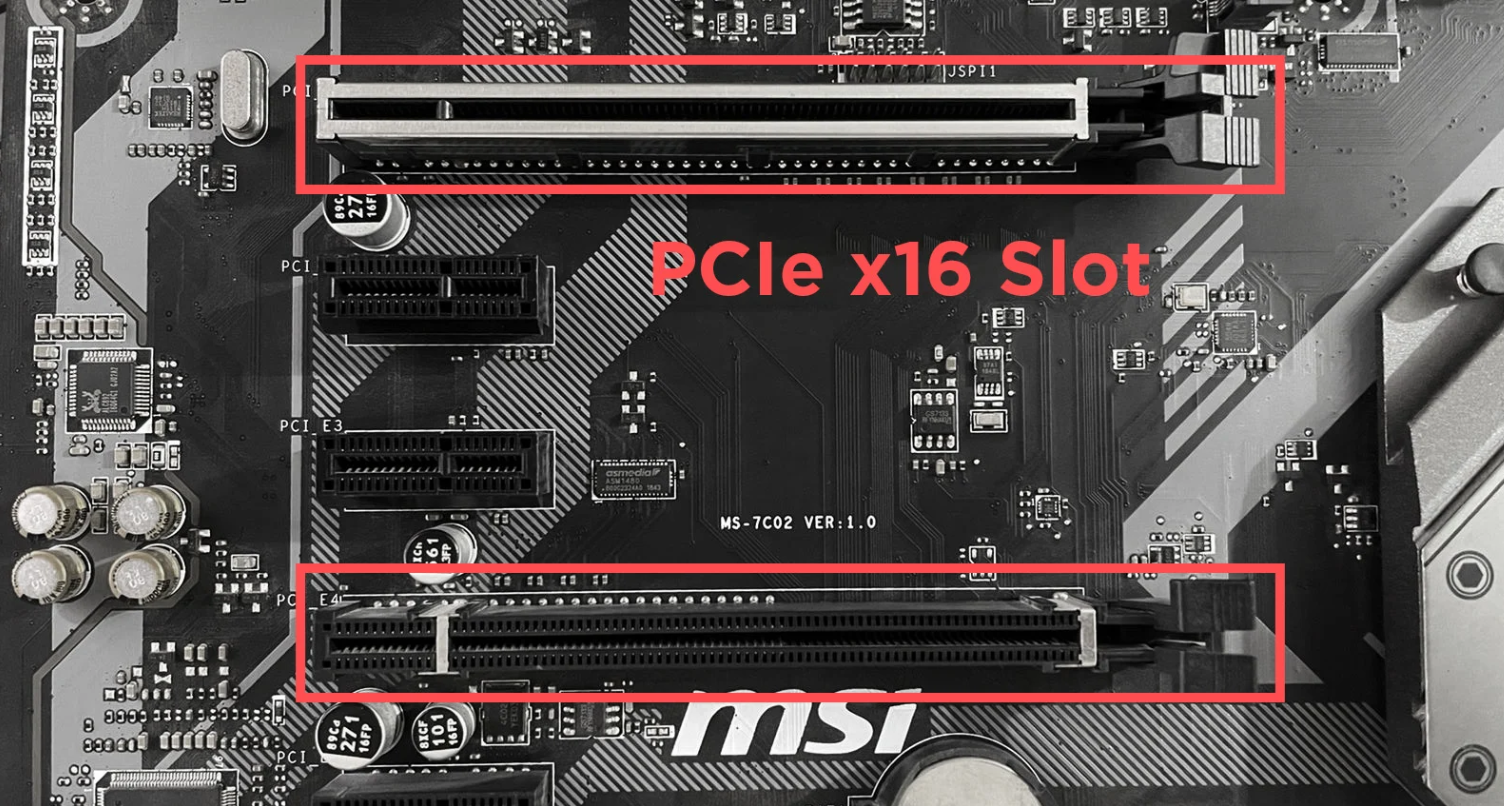
\includegraphics[width=0.8\textwidth]{pcie16.png}
\caption{PCIE X16 slots}
\label{fig:pcie16}
\end{figure}

You could use PCIE 1x risers to hold the cards in a normal computer but that would be messy and harder to manage power.

\begin{figure}[H]
\centering
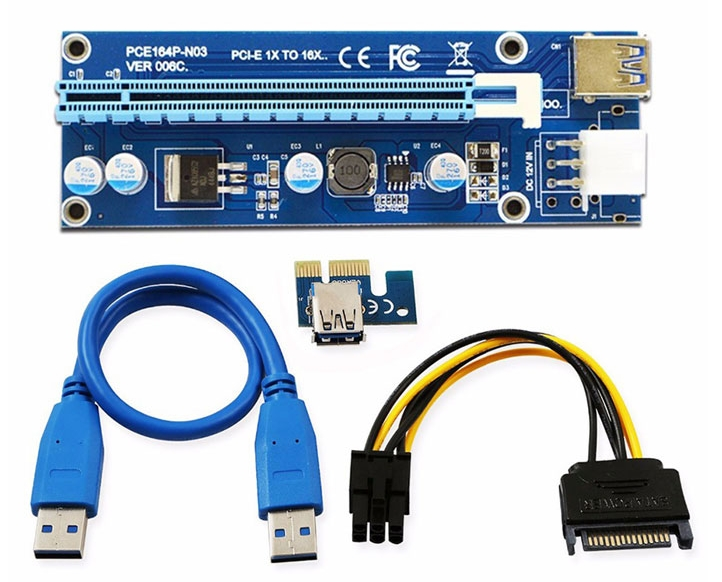
\includegraphics[width=0.4\textwidth]{riser.jpg}
\caption{PCIE 1x risers}
\label{fig:pcie1x}
\end{figure}



\begin{figure}[H]
\centering
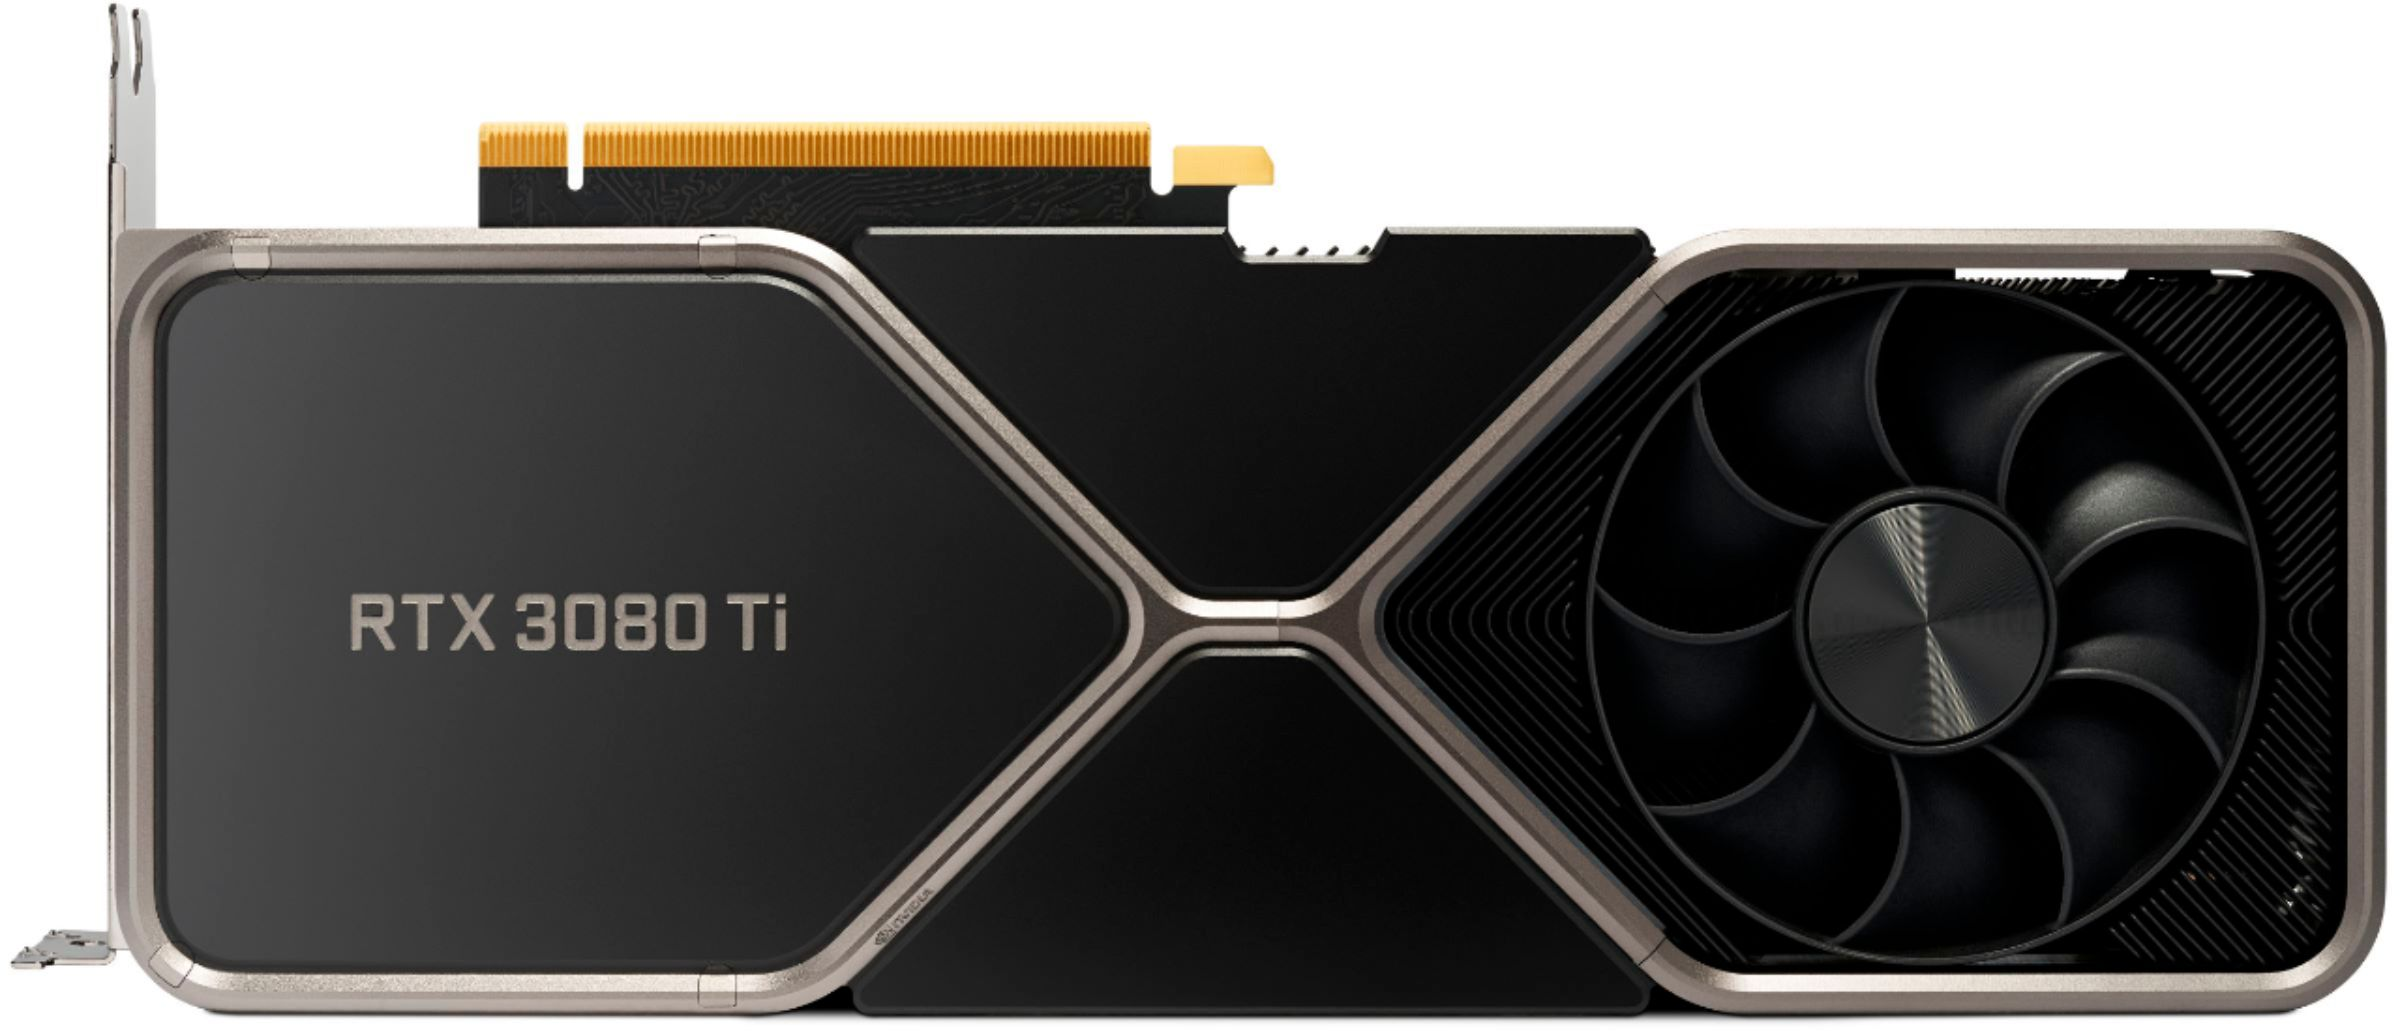
\includegraphics[width=0.4\textwidth]{6462956_sd.jpg}
\caption{RTX 3080ti}
\label{fig:rtx3080ti}
\end{figure}

To connect the cards to the motherboard you need a PCI-E slot. The PCI-E slot is a computer peripheral that is used to connect a card to a motherboard. You just connect the card into that PCIE slot.

Now a mining motherboard looks like this.

\begin{figure}[H]
\centering
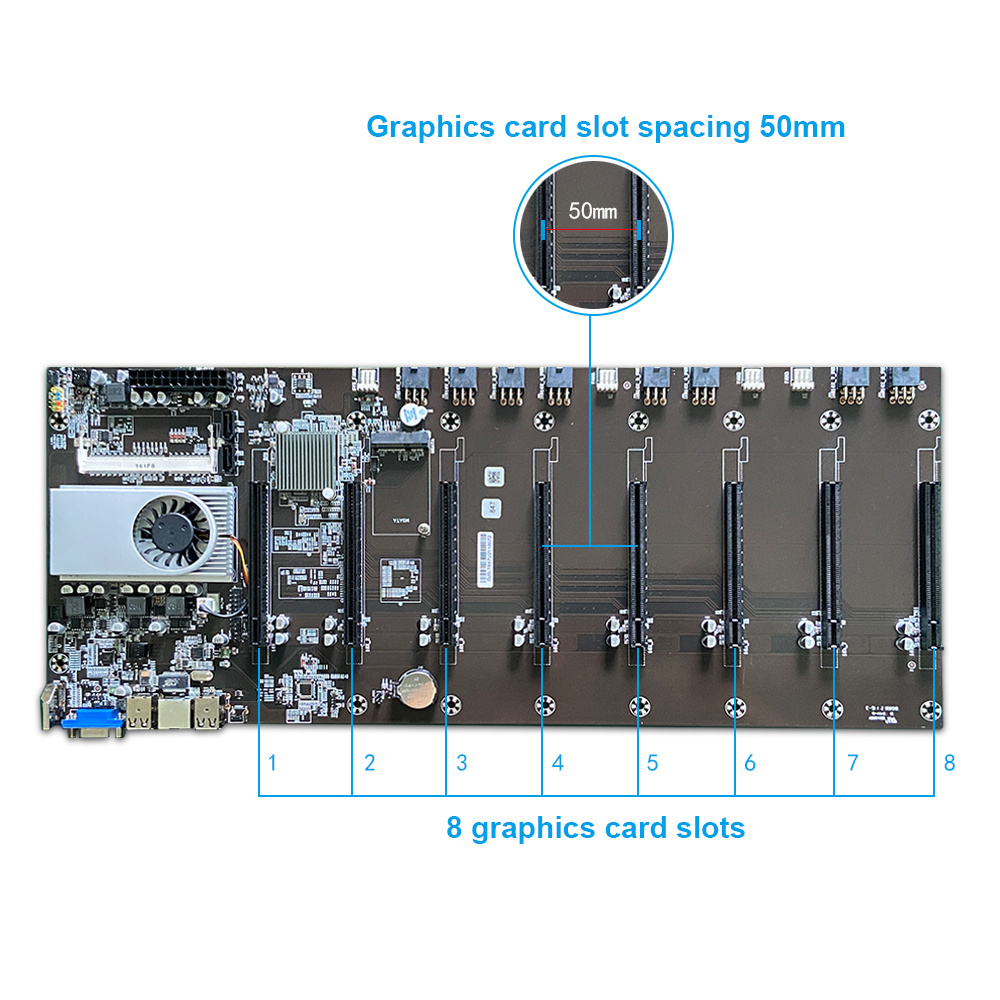
\includegraphics[width=0.8\textwidth]{miningmotherboard.jpg}
\caption{Mining Motherboard}
\label{fig:motherboard}
\end{figure}

As you can see the motherboard has 8 PCIE X16 slots. Meaning it can hold 8 cards. A normal computer can only hold one/two cards due to the size of the cards.

Let as assume the motherboard comes with a SSD, RAM , CPU built on it.

Once you have picked your motherboard you can pick your GPUs.

You could run a mixed configuration of GPUs and check out your predicted profits for each configuration.

Since we are selling our processing power to NiceHash Marketplace we will use their tool to decide our profits.

You can use this link to build your configuration of GPUs. \\

https://www.nicehash.com/profitability-calculator \\
 
It will tell you your profit $R$ which is volatile each given $t$ time. $ElectricityCost$ is the cost of electricity which is fixed.

Let us say we are building a rig for 8x RTX 3060ti cards.

As our $ElectricityCost$ is fixed we can calculate the profit for each configuration for the current BTC price. But profit changes all the time as BTC is volatile.

Note: Our rig produces a fixed hashpower for our rig. When we are mining we are mining fixed coins. Beauty of this is that we can sell our coins anytime we want for a even bigger profit.

I am going to work your through this example of a 3060ti rig which i have worked out is the most effective rig to produce.

\begin{figure}[H]
\centering
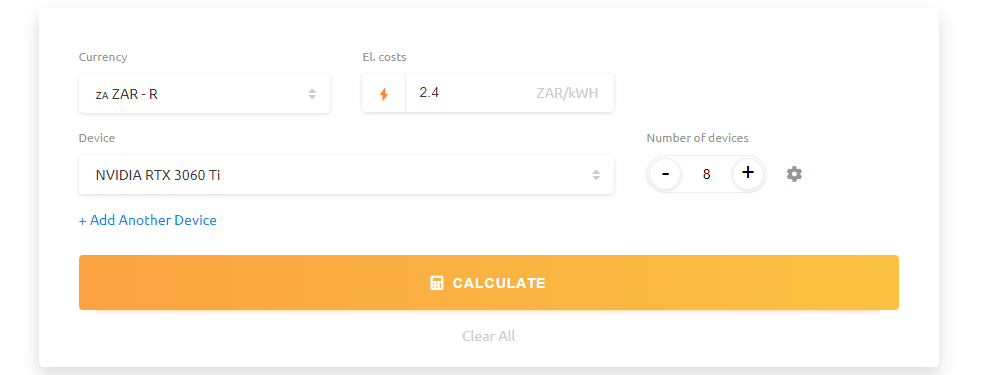
\includegraphics[width=1\textwidth]{3060tiRIG.png}
\caption{8x 3060ti Mining Rig}
\label{fig:3060ti}
\end{figure}

\begin{figure}[H]
\centering
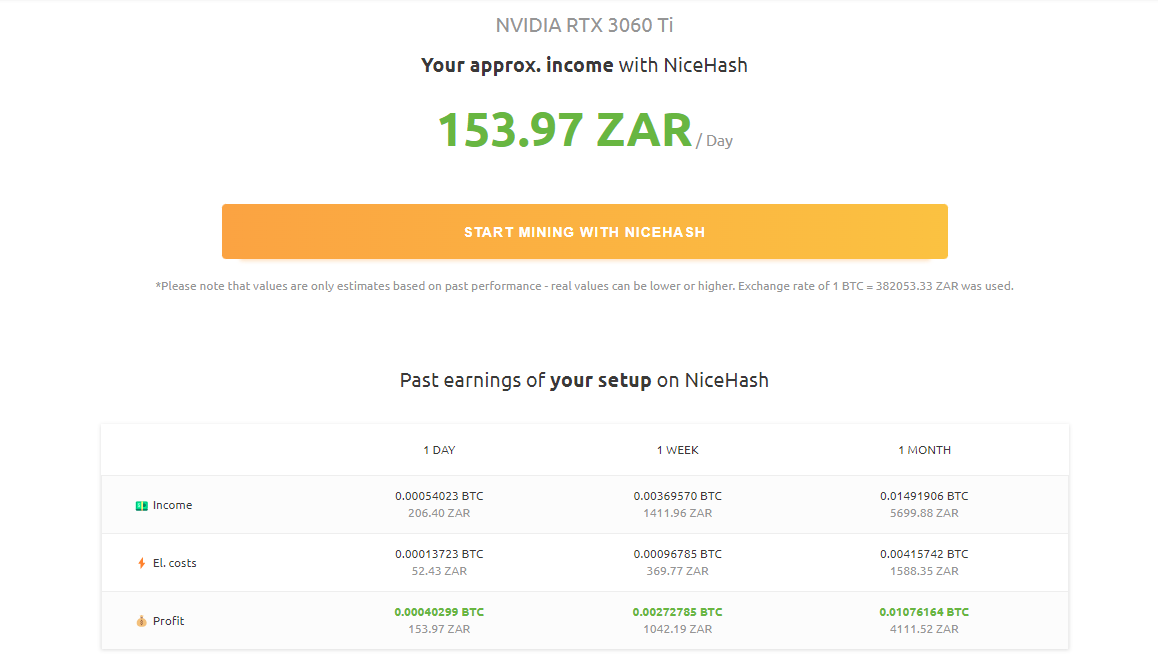
\includegraphics[width=1\textwidth]{pricechart.png}
\caption{Profitability for rig per month}
\label{fig:3060ti2}
\end{figure}

We normally use the DaggerHashimoto algorithm to mine, As it wields the best reward as per this time of writing the paper. 

\begin{figure}[H]
\centering
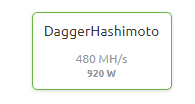
\includegraphics[width=0.35\textwidth]{algorithm.png}
\caption{DaggerHashimoto}
\label{fig:daggerhashimoto}
\end{figure}

How do we determine what PSU we should use?
As you see NiceHash predicts the power usage is 920W for the rig.

If you go online you have to check the power usage the GPUs you are using.

In this case we used all 3060ti's. As the peak power the 3060ti uses is 200W. The PSU we should go for is worked out like this.
(8x200W = 1600W) for GPU's and we could leave 400W for the motherboard and other components.

We would take a PSU that is 2000W.

Our final mining rig once done completed should look like this below. Note Nicehash had a 10 Card Rig setup.

\begin{figure}[H]
\centering
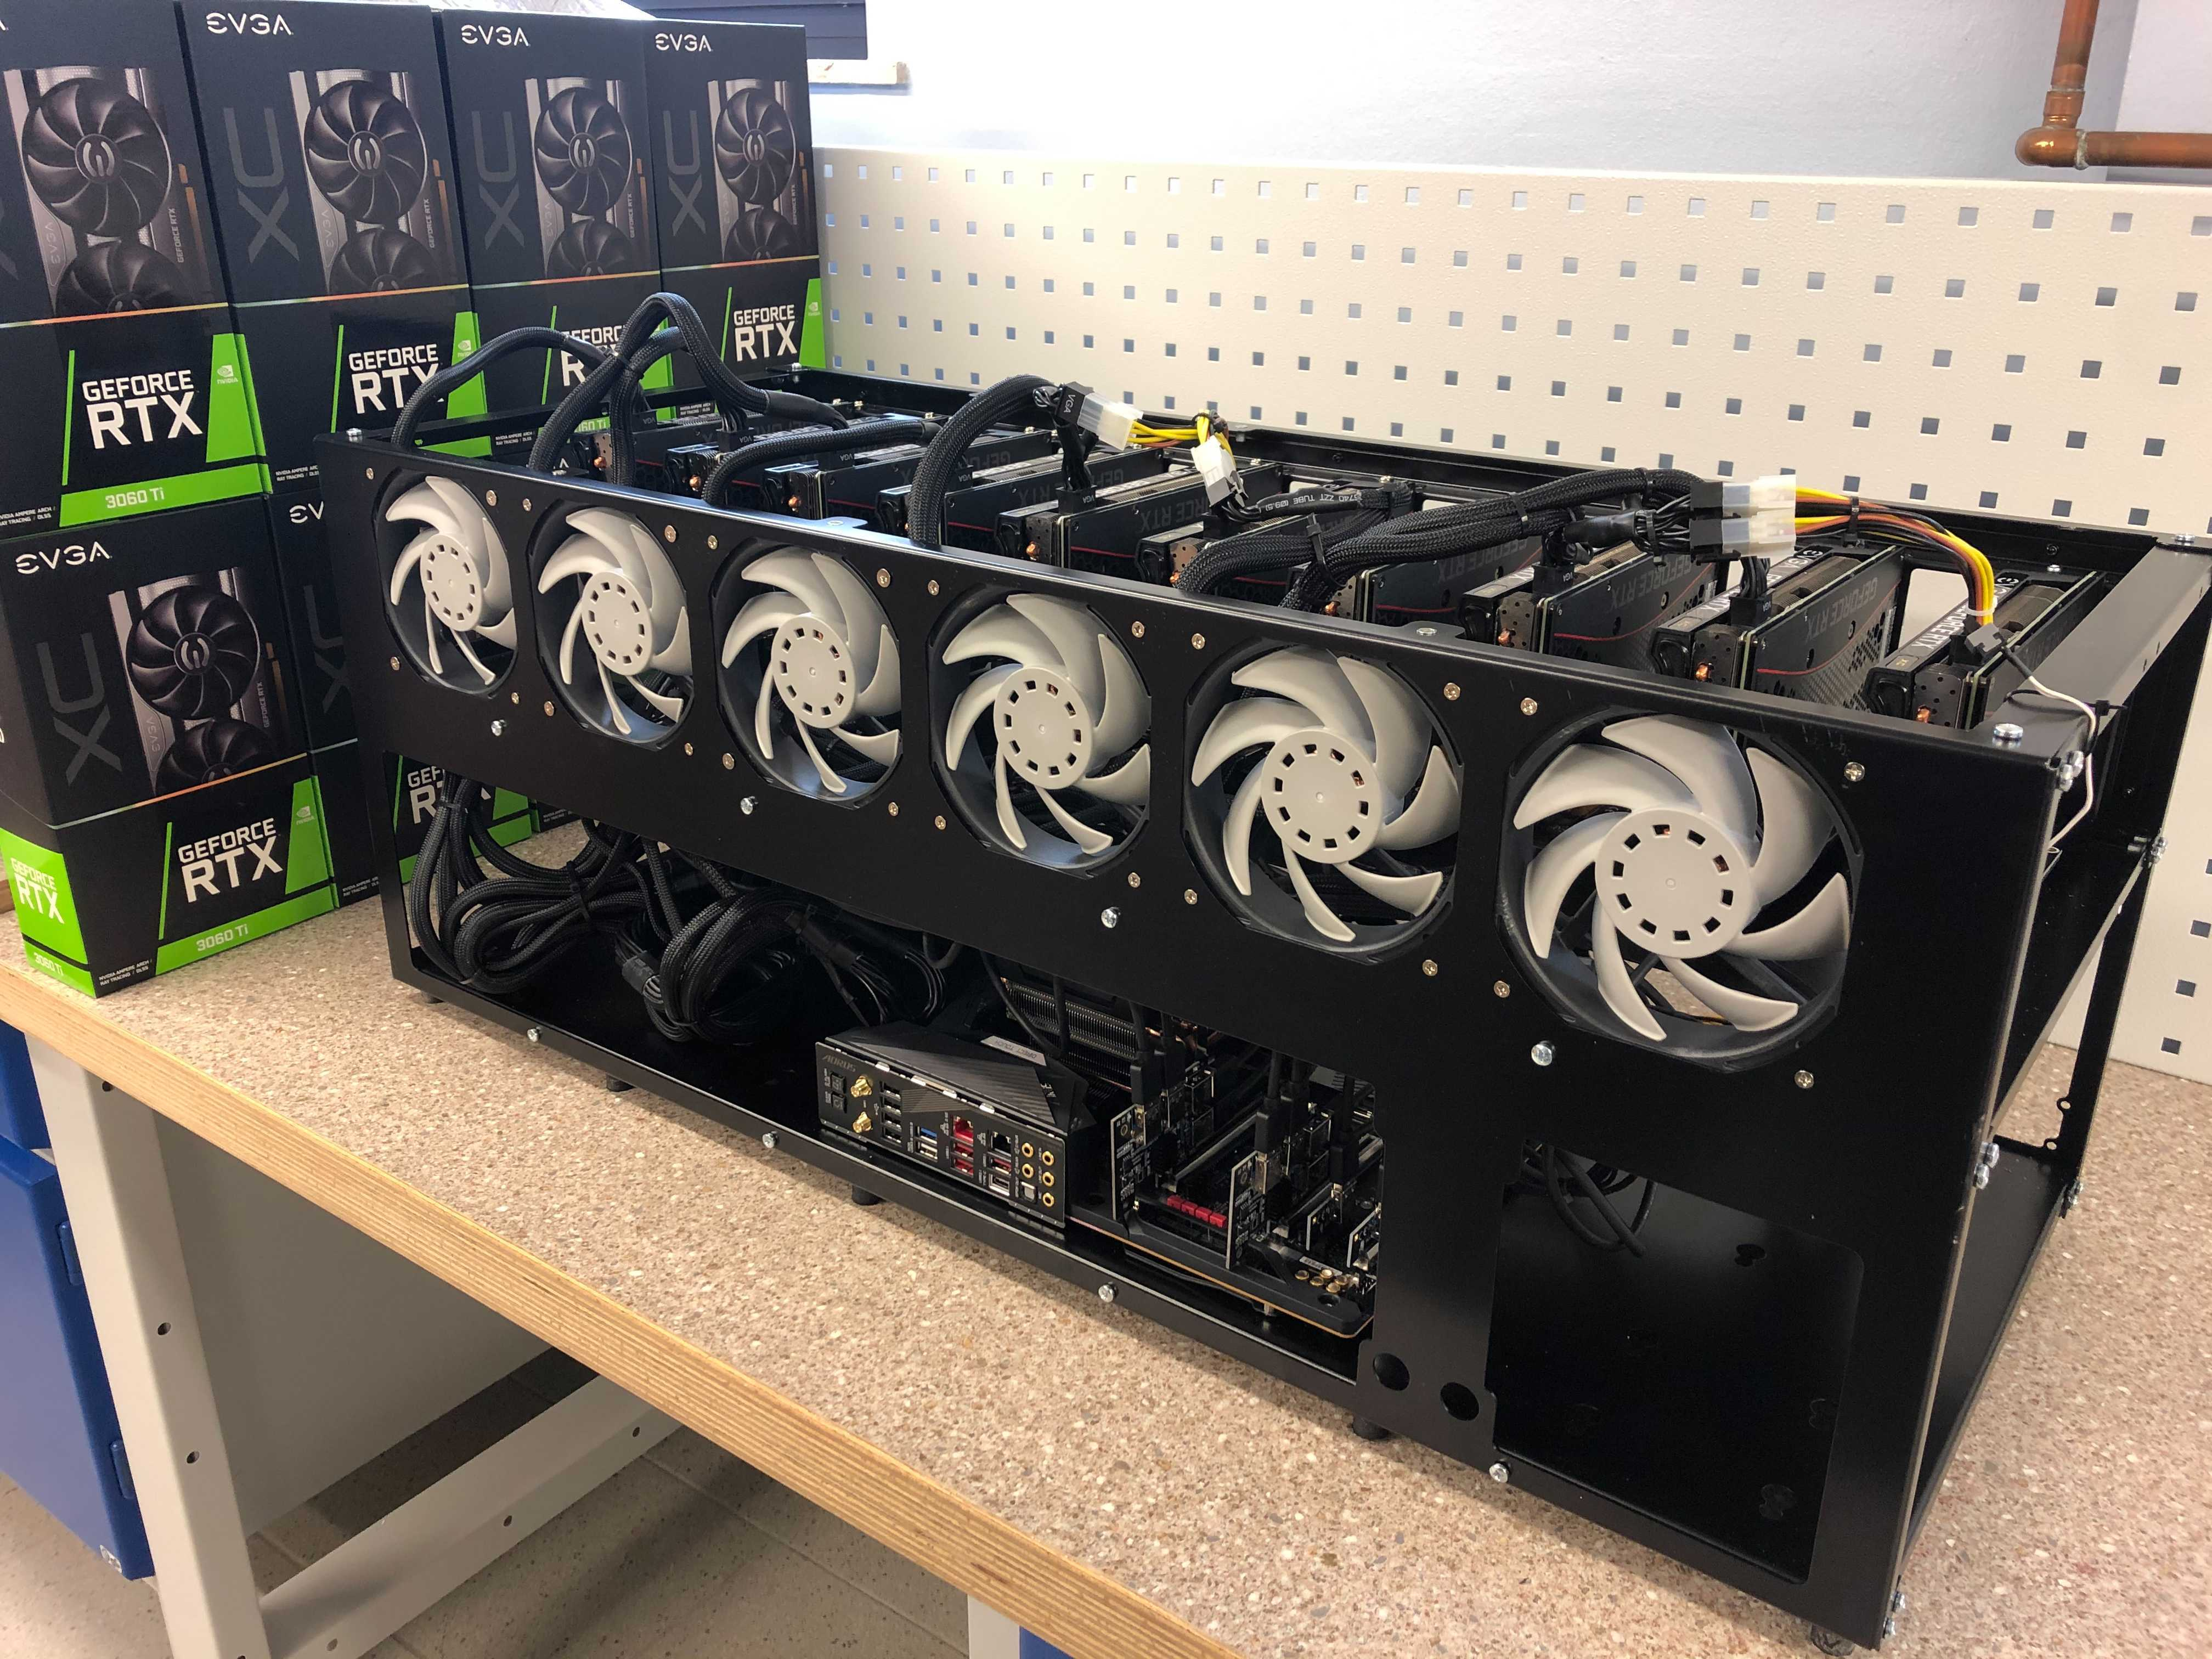
\includegraphics[width=0.8\textwidth]{nicehashrig.jpg}
\caption{NiceHash Mining Rig - https://www.nicehash.com/blog/post/the-most-profitable-mining-rig-parts-list}
\label{fig:nicehashrig}
\end{figure}

\subsection{Is it cheaper to buy a rig or build one?}

Let us use our rig of 8x Nvidia RTX 3060ti's as described earlier. \\

\begin{tabular}{ |p{6cm}||p{6cm}|}
    \hline
    \multicolumn{2}{|c|}{Building a 8x Mining Rig} \\
    \hline
    Component & Price\\
    \hline
    Motherboard,CPU,RAM Combo & R5500.00\\
    Power Supply & R3000.00\\
    Chassis & R1500.00\\
    8x Nvidia RTX 3060ti @ R8800.00 each from Wootware & R70400.00\\ 
    \hline
    Total Cost of Rig & R80400.00\\
    \hline
\end{tabular} \\ 

Now lets see what we would pay to buy that rig.

\begin{figure}[H]
\centering
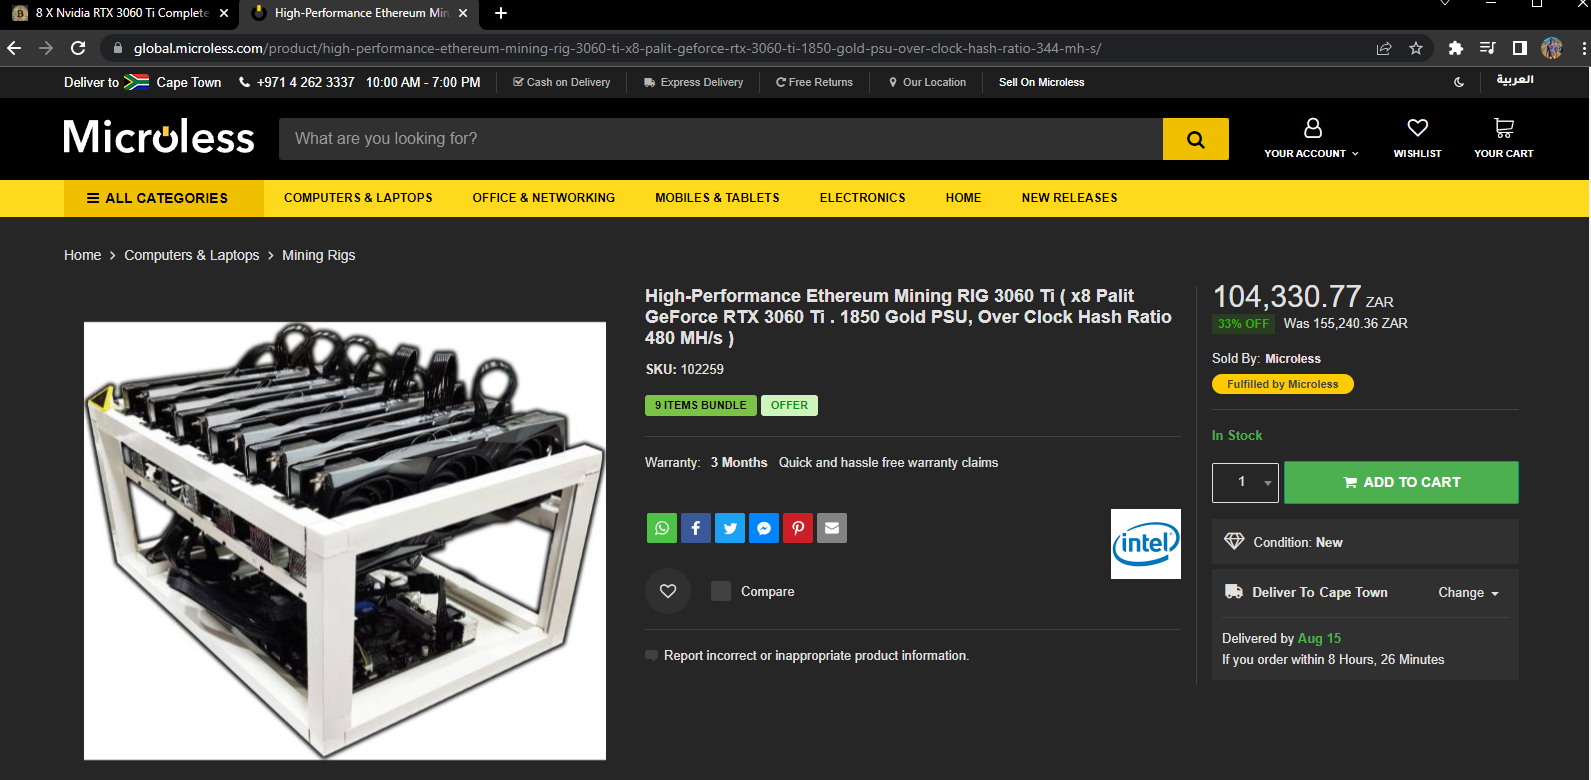
\includegraphics[width=1\textwidth]{rig1.png}
\caption{Rig Website A Cost}
\label{fig:rigcost}
\end{figure}

\begin{figure}[H]
\centering
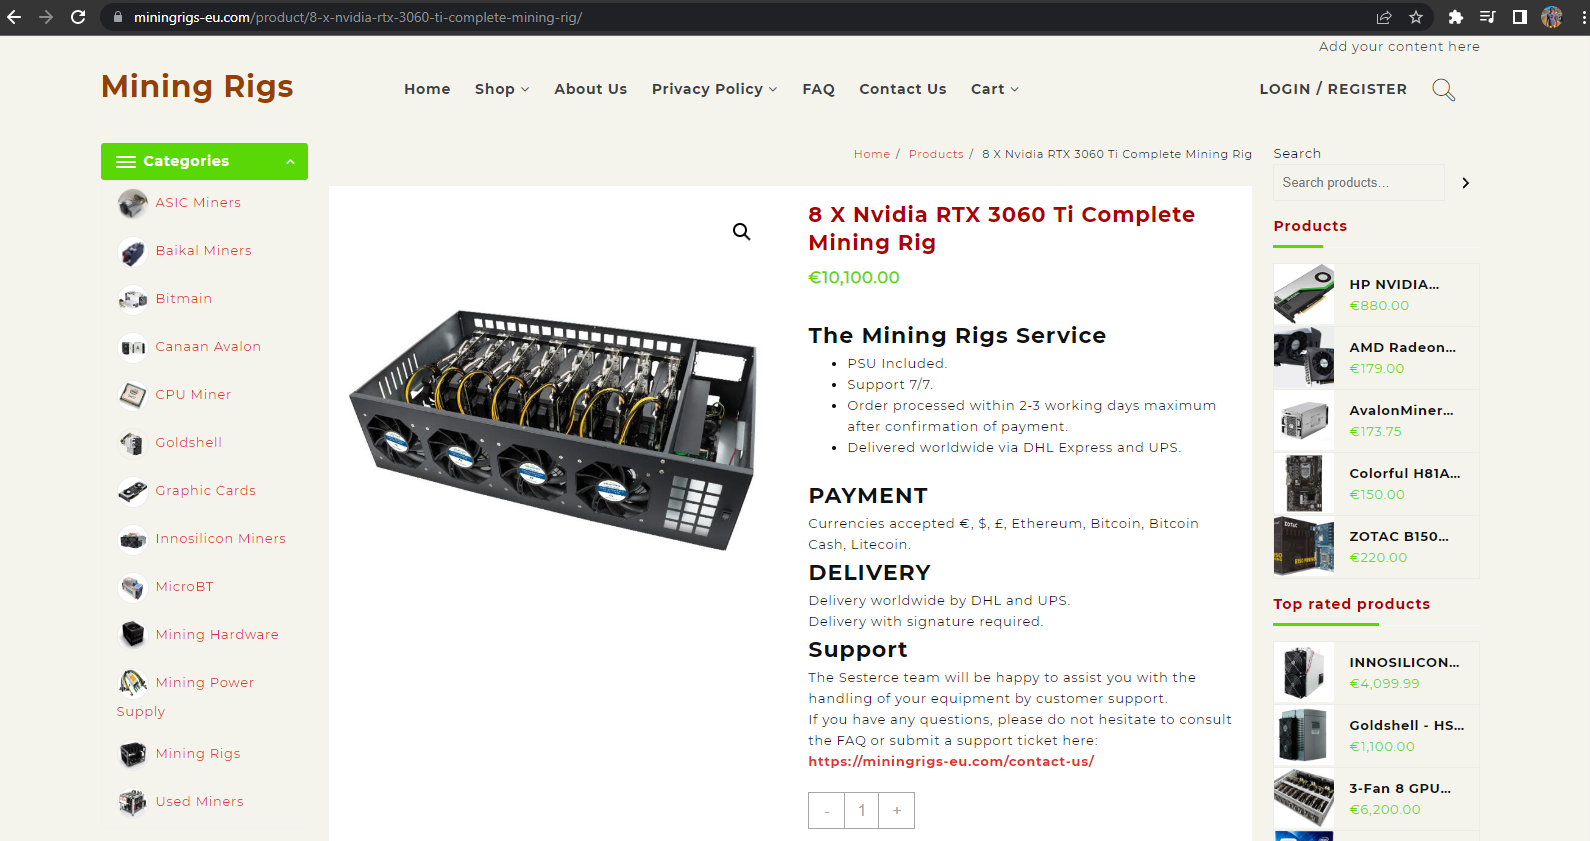
\includegraphics[width=1\textwidth]{rig2.png}
\caption{Rig Website B Cost}
\label{fig:rigcost2}
\end{figure}

\begin{figure}[H]
\centering
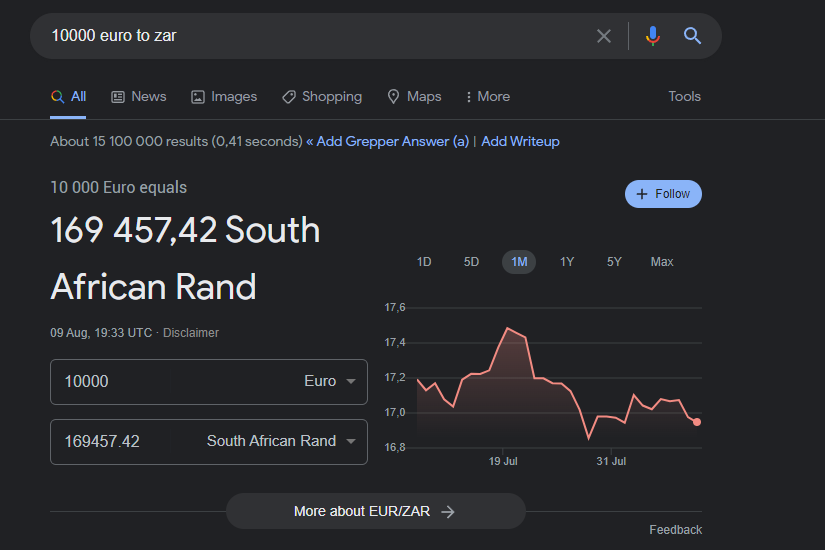
\includegraphics[width=1\textwidth]{euro.png}
\caption{10000 Euro to ZAR}
\label{fig:rigcost3}
\end{figure}


Its shocking to see Website B charge a markup of 110\% extra compared to our built rig cost.

So here we are we have concluded that we should build our rig as it is way cheaper.

\subsection{Profit and Breakeven Analysis}

Let us go back to our rig with 8x 3060ti's and see how we can break-even and make our profit.

We got 2 options for our rig.

Option A: We do nothing with the rig we just earn passive income and break even also. \\
Option B: We reinvest our money into new components to increase profit per month. \\

Let us talk about Option A first. I will assume we sell the BTC at $R500000$ \\

\begin{tabular}{ |p{2cm}||p{4cm}||p{2cm}|}
\hline
Month	&     BTC in Account&	Rand Value    \\
\hline
1	    &     0.01076164	   & 5380.82 \\
2	    &     0.02152328	   & 10761.64 \\
3	    &     0.03228492	   & 16142.46 \\
4	    &     0.04304656	   & 21523.28 \\
5	    &     0.0538082	    &26904.1 \\
6	    &     0.06456984	   & 32284.92 \\
7	    &     0.07533148	   & 37665.74 \\
8	    &     0.08609312	   & 43046.56 \\
9	    &     0.09685476	   & 48427.38 \\
10	   &      0.1076164	   & 53808.2 \\
11	   &      0.11837804	  &  59189.02 \\
12	   &      0.12913968	  &  64569.84 \\
13	   &      0.13990132	  &  69950.66 \\
14	   &      0.15066296	  &  75331.48 \\
15	   &      0.1614246	   & 80712.3 \\
16	   &      0.17218624	  &  86093.12 \\
\hline
\end{tabular} \\

As you can see it takes us 16 months to break even with our rig. \\

Option B: I took (BTC = R383376.91)\\

\begin{table}[H]    
    \begin{tabular}{|p{1cm}|p{1.4cm}||p{1.3cm}||p{2cm}||p{2cm}||p{2cm}||p{2cm}||p{3cm}|}
    \hline
        Month & Miner Income (R) & Electrcity Costs (R) @ R2.4 per kWh & Current Profit per month (R) & Miner Produced (R) & Wallet Account & Purchases (R) & Description of Purchase \\ \hline
        1 & 5722.93 & 1588.59 & 4134.34 & 4134.34 & 4134.34 & 0 & - \\ \hline
        2 & 5722.93 & 1588.59 & 4134.34 & 8268.68 & 8268.68 & 0 & - \\ \hline
        3 & 5722.93 & 1588.59 & 4134.34 & 12403.02 & 2403.02 & 10000 & Miner Rig \\ \hline
        4 & 5722.93 & 1588.59 & 4134.34 & 16537.36 & 6537.36 & 0 & - \\ \hline
        5 & 5722.93 & 1588.59 & 4134.34 & 20671.7 & 1871.7 & 8800 & RTX 3060ti \\ \hline
        6 & 6440.62 & 1787.79 & 4652.83 & 25324.53 & 6524.53 & 0 & - \\ \hline
        7 & 6440.62 & 1787.79 & 4652.83 & 29977.36 & 2377.36 & 8800 & RTX 3060ti \\ \hline
        8 & 6440.62 & 1787.79 & 4652.83 & 34630.19 & 7030.19 & 0 & - \\ \hline
        9 & 7153.67 & 1985.74 & 5167.93 & 39798.12 & 3398.12 & 8800 & RTX 3060ti \\ \hline
        10 & 7871.87 & 2185.07 & 5686.8 & 45484.92 & 284.92 & 8800 & RTX 3060ti \\ \hline
        11 & 8587.48 & 2383.72 & 6203.76 & 51688.68 & 6488.68 & 0 & - \\ \hline
        12 & 8587.48 & 2383.72 & 6799.69 & 58488.37 & 4488.37 & 8800 & RTX 3060ti \\ \hline       
    \end{tabular}
\end{table}

With this analysis we can see that we will grow our monthly profits by expanding and later on in life we need to own a crypto warehouse or even solar power this operation to cut electricity costs.



\subsection{Constraints in South Africa for crypto mining}
If you look in this country, Eskom always have load shedding. That will disrupt few hours of this operation. Some money will be lost. Later on it is necessary to get out of the grid. Get into solar power. That will offset costs and gain higher profits per month for your operation. Then as you gain more money per month it is taxable by the tax man.

\subsection{What can i do if cryptocurrency fails?}
Well you can sell/list your GPUs to gamers. I believe cryptocurrency is here to stay i dont think it will fail.

\subsection{Mining Conclusion}
In conclusion, for starting a mining business you can start small and expand operations slowly by time. You do not need to buy a rig immediately start small and grow over $t$-time. You can even start with one card at a time. The growth is up to your start up capital,investment and equipment.




        






































